\section{Theoretische Grundlagen}

In diesem Kapitel werden die grundlegenden Begriffe und Konzepte erläutert, welche wichtig für das Verständnis der Arbeit sind. Es wird zunächst der DevOps-Ansatz und das Architekturmuster der Microservices beschrieben. Anschließend wird Containervirtualisierung sowie Kubernetes erklärt.

\subsection{DevOps}

Alle der in diesem Kapitel beschriebenen Architekturmuster, Methoden und Werkzeuge lassen sich dem DevOps-Ansatz zuordnen. Für das Verständnis der Arbeit ist es also essentiell zu Verstehen was DevOps bedeutet und warum es so populär ist. Wie das Kofferwort "DevOps" bereits andeutet, beschreibt er einen Ansatz für eine effektivere und stärkere Zusammenarbeit zwischen Softwareentwicklung (Development) und IT-Betrieb (Operations). Für DevOps gibt es keine einheitliche Definition. Es ist ein Überbegriff für Denkweisen, Kultur, Methoden, Technologien und Werkzeuge. Der Kundennutzen wird dabei immer in den Mittelpunkt gestellt [\cite[S. 1]{halstenbergDevOps2020}]. Das Ziel ist es die Softwarequalität zu verbessern und die Geschwindigkeit der Entwicklung und Bereitstellung zu erhöhen [\cite[S. 6]{arundelCloud2019}]. Um die Ziele umzusetzen bedient sich DevOps etablierten Methoden und Werkzeuge um daraus einen ganzheitlichen Ansatz zu formulieren. \\
\\
DevOps wird immer wichtiger, da durch das Aufkommen von Cloud Computing die Entwicklung und der Betrieb von Anwendungen nicht mehr trennbar ist. DevOps in ein Unternehmen einzuführen ist ein langwieriger Prozess, da insbesondere die Unternehmenskultur transformiert werden muss. Vor allem in großen Unternehmen zeigt sich das viele Prozesse schwerfällig geworden sind und nicht mehr dem eigentlichen Kundennutzen dienen. DevOps soll dieses Problem lösen und Unternehmen wieder anpassungsfähiger machen, ohne geordnete Strukturen zu verlieren.

\begin{figure}[H] 
    \centering
    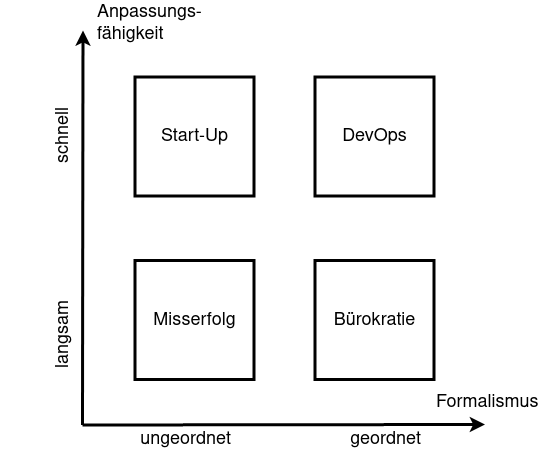
\includegraphics[width=0.6\textwidth]{figures/DevOpsDiagramm.png}
    \caption{Kategorisierung von Unternehmen [\cite[S. 11]{halstenbergDevOps2020}]}
\end{figure}

Eine reduzierte Time-to-Market kann durch engere Abstimmung und Automatisierung erreicht werden. Die Time-to-Market gibt an, wie lange es dauert eine Änderung zum Kunden, also auf die Produktionsumgebung, zu bringen. So können Änderungen schnell ausgeliefert werden und Feedback vom Endanwender erreicht schneller die Entwickler. Zur Umsetzung können Methoden wie Continuous-Integration und Continuous-Delivery eingesetzt werden, aber auch Architekturmuster wie Microservices und Werkzeuge wie Docker und Kubernetes können dabei unterstützen.

\subsection{Microservices}

Im Mittelpunkt dieser Arbeit stehen Microservices. Bei Microservices handelt es sich um ein Architekturmuster zur Modularisierung von Software (\cite[S. 15]{newmanMicroservices2015}). Eine einheitliche Definition für Microservices gib es nicht [\cite[S. 2]{wolffMicroservices2018}]. Bei der Beschreibung von Microservices werden grundlegende Prinzipien einer standardisierten Definition vorgezogen. \\
\\
Microservices sind das Gegenteil von klassischen monolithischen Softwarearchitekturen. Ein Monolith ist eine einzelne, zusammenhängende und untrennbare Einheit. Die Erweiterbarkeit und Wartbarkeit von Monolithen ist häufig komplex, da die Codebasis umfangreich ist und mit der Zeit immer stärker wächst. Die Arbeit von mehreren Entwicklerteams ist ineffizient, dar ein höher Abstimmungsbedarf nötig ist. Des Weiteren lässt ist die Skalierbarkeit des schwergewichtigen Monolithen sehr beschränkt. Durch Modularisierung einer Anwendung lassen sich diese Probleme abschwächen, können jedoch nicht komplett behoben werden.

\begin{figure}[H] 
    \centering
    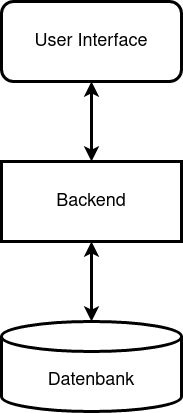
\includegraphics[width=0.2\textwidth]{figures/Monolith.png}
    \caption{Beispielhafter Aufbau einer monolithischen Architektur}
\end{figure}

Genau hier setzten Microservices an. Obwohl der Begriff Microservices noch realtiv jung ist, sind die dahinterstehenden Konzepte bereits deutlich älter [\cite[S. 15]{newmanMicroservices2015}]. Zur Verständlichkeit und leichteren Weiterentwicklung werden große Systeme werden schon lange in kleine Module unterteilt. Die Besonderheit von Microservices liegt darin, dass die Module einzelne Programme sind. Das Architekturmuster der Microservices zählt zu den verteilten Systemen. Die einzelnen Microservices laufen zumeist auf vielen unterschiedlichen Rechnern und kommunizieren über das Netzwerk.

\begin{figure}[H] 
    \centering
    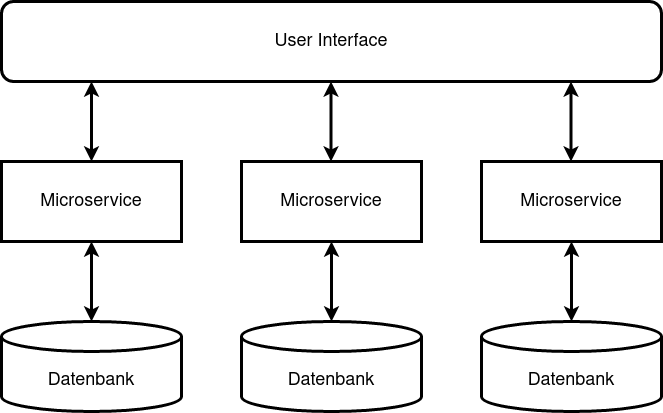
\includegraphics[width=0.71\textwidth]{figures/Microservices.png}
    \caption{Beispielhafter Aufbau einer Microservice-Architektur}
\end{figure}

Ein einzelner Microservice soll eine Aufgabe bestmöglich erledigen. Dieser Ansatz ist angelehnt an die \acs{UNIX}-Philosophie: "Mache nur eine Sache und mache sie gut" [\cite[]{salusQuarter1994}]. Jeder Microservice bildet so eine klar definierte Funktion des Gesamtsystems ab. Die Microservices müssen eigenständig sein, sodass sie unabhängig voneinander verändert und bereitgestellt werde können. Die Kommunikation zwischen den Microservices erfolgt ausschließlich über das Netzwerk mittels sprachunabhängiger Schnittstellen, sogenannte \acp{API} [\cite[S. 64]{trempArchitekturen2021}]. \\
\\
Die Größe eines Microservices ist nicht zwangsläufig entscheidend [\cite[S. 2]{wolffMicroservices2018}]. Der Name "Microservices" deutet bereits an, dass es sich um kleine Services handelt, jedoch ist eine genaue Festlegung der Größe nicht sinnig [\cite[S. 22]{newmanMicroservices2015}]. Eine Messung der Größe durch die Anzahl der Codezeilen wäre zwar denkbar, jedoch hängen derartige Kriterien stark von der verwendeten Programmiersprache ab. Stattdessen sollte sich die Größe an fachliche Gegebenheiten anpassen. Je kleiner die Services gestaltet werden, umso stärker kommen die in den nachfolgenden Abschnitten beschriebenen Vor- und Nachteile zur Geltung. Eine Obergrenze für die Größe eines Microservices stellt die Teamgröße dar. An einem Microservice darf immer nur ein Entwicklerteam arbeiten [\cite[S. 23]{newmanMicroservices2015}]. Kann der Microservice nicht mehr von einem Team alleine entwickelt und gewartet werden, so ist er zu groß. Ein Microservice sollte auch nur so groß sein, dass er von einem Entwickler allumfassend verstanden werden kann. Ein Microservice sollte jedoch auch nicht zu klein gewählt werden, da ansonsten der Aufwand für die Bereitstellung der vielen Microservices sehr groß wird und die Kommunikation über das Netzwerk ansteigt. \\
\\
Um von Microservices zu profitieren müssen Strukturen in Unternehmen überarbeitet werden. Das Gesetz von Conway besagt, dass durch die Kommunikationsstrukturen einer Organisation auch die Struktur der Systeme, welche die Organisation entwirft, vorgegeben wird [\cite{conwayHow1968}]. Bei monolithischen Anwendungen werden die Entwicklerteams häufig nach ihrem Fachbereich aufgeteilt. Es bilden sich so beispielsweise Teams spezialisiert auf das Frontend, das Backend und die Datenbank. Die entwickelte Anwendung wird, nach dem Gesetz von Conway, auch aus diesen drei Bereichen bestehen. Wenn nun ein neues Feature umgesetzt werden soll, müssen sich alle drei Teams miteinander absprechen. Um eine Microservice-Architektur umzusetzen muss also auch die Struktur des Unternehmens verändert werden. Die Entwicklerteams müssen crossfunktional mit Spezialisten aus verschiedenen Fachbereichen aufgebaut werden. Der Vorteil ist das Änderungen so häufig nur ein Entwicklerteam betreffen und der Koordinationsaufwand sinkt. \\
\\
Microservices werden häufig mit \ac{SOA} in Verbindung gebracht. Microservices übernehmen viele Prinzipien von \ac{SOA}. \ac{SOA} ist ein Ansatz mit dem Ziel Funktionalitäten von betrieblichen Anwendungen durch Services von außerhalb zugreifbar zu machen [\cite[S. 2]{wolffMicroservices2018}]. Ein Service bildet in diesem Kontext einen Geschäftsprozess ab. Dadurch soll Flexibilität und Wiederverwendbarkeit in der IT von Unternehmen erhöht werden. Es gibt also durchaus viele Parallelen zu Microservices, jedoch setzen sie an verschiedenen Ebenen an. Während Microservices ein konkretes Architekturmuster für ein einzelnes System ist, beschreibt \ac{SOA} wie viele Systeme in einem Unternehmens miteinander interagieren können. \\
\\

\subsubsection{Vorteile}

Das Aufteilen von Software bringt wichtige Vorteile mit sich.

\paragraph{Modularisierung}
Bei klassischen Software-Monolithen, welche aus Komponenten zusammengestellt wird, entstehen schnell unerwünschte Abhängigkeiten. Die viele Abhängigkeiten erschweren die Wartung oder Weiterentwicklung. Da die einzelnen Microservices eigene Programme sind, herrscht eine starke Modularisierung. Die Programme sind eigenständig und kommunizieren nur über explizite Schnittstellen. Ungewollte Abhängigkeiten entstehen hier deutlich schwerer. (\cite[S. 3]{wolffMicroservices2018})

In der Praxis wird die Architektur von Deployment-Monolithen meistens zunehmend schlechter. (\cite[S. 3]{wolffMicroservices2018})

\paragraph{Austauschbarkeit}
Da Microservices nur über eine explizite Schnittstelle genutzt werden, können sie einfach durch einen Service, der die selbe Schnittstelle anbietet ersetzt werden. Bei der Ersetzung ist der neue Service nicht an den Technologie-Stack des alten Service gebunden. Auch die Risiken werden geringer, da bei schwerwiegenden Fehlentscheidungen in der Entwicklung, ein Austausch mit weniger Aufwand verbunden ist. (\cite[S. 4]{wolffMicroservices2018})

Sie können auch deutlich schneller eingesetzt werden. (Time to Market)

Das gesamte neu schreiben eines Microservices ist in der Regel nicht besonders schwer. Viele Unternehmen scheitern an der Wartung oder Erweiterungen von alten monolithischen Systemen (\cite[S. 29]{newmanMicroservices2015}). Da Problem ist das die Ablösung dieser großen Systeme eine fast unmöglichen Mammutaufgabe ist.

\paragraph{Skalierbarkeit}
Durch die Unabhängigkeit der Microservices können sie auch unabhängig voneinander skaliert werden. So kann eine einzelne Funktionalität, welche stärker genutzt wird, skaliert werden, ohne das gesamte System zu skalieren. (\cite[S. 5]{wolffMicroservices2018})

Dadurch können gezielt Falschenhälse in der Anwendung entsprechend hochskaliert werden.

Beim Einsatz von Cloudanbietern wie AWS ist es möglich eine Skalierung nach dem genauen Bedarf vorzunehmen. So wird nur die tatsächlich Gebrauchte Leistung des Systems bezahlt. Aber auch bei on-Premise Lösungen profitiert man von einer effektiveren Lastausnutzung. Auch die Verteilung der Last ist einfacher, da die Services auf unterschiedlichen Maschinen laufen. 

Es gibt wenige Architekturmuster wie dieses, welche so eng mit Kosteneinsparungen verbunden sind. (\cite[S. 27]{newmanMicroservices2015}).

\paragraph{Technologiefreiheit}

Des Weiteren führt die Unabhängigkeit auch zu einer großen Technologiefreiheit. Die verwendeten Technologien müssen schließlich nur in der Lage sein die explizite Schnittstelle anzubieten. (\cite[S. 5]{wolffMicroservices2018})

Statt auf einen Technologie-Stack als Kompormiss zu verwenden, kann für jeden Service die am besten geeigneten Technologien ausgewählt werden. 

Außerdem können neue Technologien auch leichter angewendet werden. Bei einer großen monolithischen Anwendung ist eine Umstellung auf beispielsweise ein neue Programmiersprache ein schwieriger und langwieriger Prozess. Bei Microservices kann die neue Sprache zuerst an einem einzelnen Service getestet werden und dann schrittweise das ganze System umgestellt werden. Oder eben nur die Services für welche die neue Sprache auch wirklich Vorteile besitzt. (\cite[S. 25]{newmanMicroservices2015}).

Ein Nebeneffekt von dieser Technologiefreiheit ist auch, dass die Auswirkungen von falschen Entscheidungen über die Einführung von neuen Technologien deutlich reduziert. 


\paragraph{Continuous Delivery}

Ein wesentlicher Grund für die Einführung ist Continuous Delivery. Die kleinen Microservices können leichter deployt werden und das Deployment bietet weniger Gefahren und ist einfacher abzusichern, als bei einem Monolithen. (\cite[S. 5]{wolffMicroservices2018}) \\
\\
Das schnelle und größtenteils automatisierte Ausliefern von Software ist wichtig. In der der schnelllebigen Zeit ist man nur im Vorteil wenn neue Features und Fehlerbehebungen so schnell wie ihren Weg zum Benutzer finden. Microservices können schneller und leichter deployt werden als große Monolithen. Vor allem bei geringen Änderungen von einigen Codezeilen ist der gesamte Deployment Prozess von Monolithen sehr nervig.

Durch Ihre Unabhängigkeit können nur einzelne Services nach Änderungen neu bereitgestellt werden. Auch hier ist sind die Auswirkungen von Fehlern geringer. Ist eine Auslieferung fehlerhaft ist nicht das ganze System davon betroffen, sondern lediglich ein Service. Auch kann bei Microservices leicht noch eine alte Version desselben Services betrieben werden, bis die fehlerfreie Funktion der neuen Version gewährleistet ist. Bei einem Monolithen wäre der Ressourcenverbrauch in so einem Fall doppelt so hoch, wie die eigentliche Anwendung benötigt. \\

\subsubsection{Herausforderungen}

Doch natürlich haben Microservices wie jedes Architekturmuster auch einige Nachteile. Die Aufteilung eines Systems in viele Microservices erhöht die Komplexität. 

\paragraph{Versteckte Beziehungen}

Die Beziehungen von Microservices können schnell unüberschaubar werden. Ob und welche Funktionen ein Microservice von anderen Microservices in Anspruch nimmt sind nicht direkt ersichtlich. Ein genaues Monitoring ist hierbei nötig. Auch auf Code-Ebene kann es zu ungewollten Abhängigkeiten kommen, wenn mehrere Microservices die selbe Bibliothek verwenden. Unter Umständen müssen bei Änderungen an dieser Bibliothek die Services gemeinsam ausgeliefert werden und die Unabhängigkeit geht verloren (\cite[S. 75]{wolffMicroservices2018}).

\paragraph{Refactoring}

Während bei Softwaremodulen leicht Teile des Codes von einem Modul in ein anderes verschoben werden können ist es bei Microservices deutlich schwieriger. Wenn eine Funktionalität in einen anderen Microservice verschoben werden muss, dann ist ein höherer Aufwand erforderlich. Deshalb ist es wichtig die Makro-Architektur von Microservices mit bedacht zu wählen. Änderungen auf dieser Ebene sind im Nachhinein deutlich aufwendiger.

\paragraph{Architektur}

Die Architektur ist wichtiger als bei anderen Systemen.

\paragraph{Betrieb}



\paragraph{Verteilte Systeme}

Microservices sind verteilte Systeme und bringen auch die damit verbundenen Nachteile mit sich. Da die Kommunikation mit den Microservices über das Netzwerk läuft, ist die Antwortzeit der Microservices von der Latenz abhängig. Da wird vor allem dann problematisch wenn ein Microservice viele Dienste von anderen Microservices in Anspruch nimmt. Deshalb sollten Microservices untereinander möglichst wenig kommunizieren müssen. Besitzen zwei Microservices viele Abhängigkeiten, kann dies ein Hinweis auf eine falsche Einteilung der Microservices sein. Des Weiteren muss das Netzwerk die höhere Last durch die Aufrufe standhalten. Außerdem ist Kommunikation über das Netzwerk immer unzuverlässig.

\paragraph{Technologie-Komplexität}

Die technologische Freiheit der Microservices kann schnell zu einer Herausforderung werden. Wenn jeder Microservice einen komplett unterschiedlichen Technologie-Stack verwendet, steigt die Komplexität des Gesamtsystems. Auch wird der Wechsel von Mitarbeitern zu anderen Teams schwieriger. Es bietet sich also an den Technologie-Stack einzuschränken und übergreifende Richtlinien für alle Microservices zu bestimmen.

\subsubsection{Architektur}

Die Architektur bei Micrservices ist das Finden von Kompromissen. Die einzelnen Entwicklerteams sollten viel Freiheit haben, um die nach ihrer Meinung am Besten geeigneten Technologien für ihren Service zu verwenden. Es macht jedoch Sinn gewisse Vorgaben und Rahmenbedingungen vorzugeben. Die Beschränkung auf eine Auswahl von beispielsweise fünf Programmiersprachen macht Sinn, um Wissen nicht zu weit zu verstreuen. Für die Schnittstellen ist es sinnvoll einige wenige Schnittstellenarten festzulegen, die von allen Services verwendet wird.  \\
\\
Die Mikroarchitektur, also die Architektur mit der ein einzelner Service implementiert wurde, sollte von außen nicht sichtbar sein und besitzt somit für das Gesamtsystem keine Relevanz. \\
\\
Die fachliche Archtiektur, also die Aufteilung in verschiedene Bereiche, die jeweils von einem Microservice umgesetzt werden. Wo bei dieser Aufteilung die Grenzen gezogen werden ist eine der zentralen Herausforderungen (\cite[S. 102]{wolffMicroservices2018}). Das entscheidende Kriterium für die Aufteilung ist, dass Änderungen möglichst nur einen Service betreffen und somit von nur einem Team durchgeführt werden können. Dadurch ist wenig Abstimmung zwischen den Entwicklerteams notwendig und die Vorteile der Microservices kommen erst richtig zur geltung. Jeder Microservice solle also eine fachlichen Kontext darstellen, der eine abgeschlossene Funktionalität darstellt. \\
\\
Natürlich sind die Microservices nie vollständig voneinander unabhängig. Es wird Services geben die, die Funktionalität anderer Services aufrufen. Zu viele solcher Verbindungen führen jedoch zu einer hohen Abhängigkeit und widersprechen dem Microservice-Ansatz. Eine lose Kopplung, also nur wenige Abhängigkeiten sind erstrebenswert, da so sich Änderungen so nur auf einen Service auswirken. Benötigt ein Microservice viele Funktionalitäten von einem anderen Microservice kann das ein Hinweis auf eine schlechte Aufteilung sein und die Services sollten an einer anderen Stelle aufgeteilt werden oder womöglich direkt zusammen gelegt werden. Innerhalb eines Micrservice sollten die Komponenten und Module des Programms jedoch eine starke Kopplung besitzen. Dadurch wird gewährleistet, dass die Bestandteile wirklich zusammengehören. \\
\\
Zyklische Abhängigkeiten sind auch zu vermeiden, da dort ohne weitere Abstimmung Änderungen in einem der beiden Services nicht möglich sind. \\
\\
Eine bewährter Ansatz für den Anfang der Architektur ist es, mit großen Service zu beginnen und diese aufzuteilen. Einen großen Service aufzuteilen ist einfach. Die Gesamtarchitektur von vielen kleinen Services zu überarbeiten jedoch sehr komplex. \\

Herausforderung: Microservice-Systeme sind schwer änderbar (auf Makro Ebene)

Architektur eines Microservice: Erklärung Schichtenarchitektur, wenige Vorgaben, wird vom Team gehandhabt

\subsubsection{Integration und Kommunikation}

Microservices müssen miteinander kommunizieren. Die Integration der Services ist auf drei verschiedenen Ebenen denkbar.

\paragraph{UI}

\paragraph{Datenbank}

\paragraph{Microservices}

Zuletzt müssen natürlich auch Microservices direkt miteinander kommunizieren, um so Funktionalität von anderen Services aufzurufen. Die meist verbreitetste Technologie ist HTTP REST. Es gibt auch weitere Ansätze wie SOAP oder Message-Systeme.

{Definition REST}


\subsubsection{Bereitstellung und Betrieb}



\subsubsection{Fazit}

Viele Vorteile
Wichtige Dinge um die sich gekümmert werden müssen: Skalierung, Deployment, Service Discovery werden durch Kubernetes übernommen und erleichtert.


\subsection{Docker}

Anwendungen mit Microservice-Architektur verwenden heutzutage häufig Containervirtualisierung zur Bereitstellung. Durch die leichtgewichtige Containervirtualisierung können mehrere isolierte Instanzen eines Betriebssystem auf dem selben Kernel ausgeführt werden. Dadurch sind die Container ressourcenschonender als die Virtualisierung mittels Hypervisor, bei dem jede virtuelle Maschine sein eigenes Betriebssystem ausführt.

\begin{figure}[H] 
    \centering
    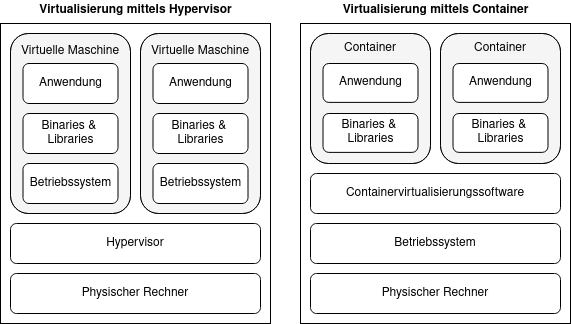
\includegraphics[width=0.95\textwidth]{figures/containervirtualisierung.png}
    \caption{Vergleich Virtualisierung mittels Hypervisor und Container}
\end{figure}

Für die Ausführung einer Anwendung werden Abhängigkeiten wie Bibliotheken, Compiler und Interpreter benötigt. Des Weiteren muss die Anwendung richtig konfiguriert werden. Vor allem bei einer Microservice-Architektur kann das ein Problem werden, da die Microservices über große Netzwerke verteilt auf verschiedenartigen Rechnern bereitgestellt werden sollen. Containervirtualisierung löst dieses Problem, mit einem standardisierten Image-Datei, das die Anwendung mitsamt aller Abhängigkeiten und Konfigurationen beinhaltet [\cite[S. 9]{arundelCloud2019}]. Diese Image-Datei läuft unabhängig von der Plattform auf jedem Rechner, sofern die zugehörige Containervirtualisierungssoftware installiert ist. \\
\\
Eine freie Software zur Containervirtualisierung ist Docker. Docker ergänzt die Containervirtualisierung mit benutzerfreundlichen Werkzeugen  und ist der Branchenstandard für Containervirtualisierung. Im Folgenden werden die wichtigsten Begriffe und Funktionen von Docker näher beschrieben. \\
\\

\subsection{Docker Image}

Ein Docker Image ist das Speicherabbild eines Containers. Das Image beinhaltet alle Informationen, die zum Starten eines Containers notwendig sind.  Bei Docker besteht das Image aus mehreren Schichten. Jede Schicht repräsentiert eine Abhängigkeit oder Konfiguration, welche für die Anwendung benötigt wird. Docker optimiert automatisch den verwendeten Speicherplatz durch Wiederverwendung, wenn zwei Images eine gleiche Schicht verwenden. Die Docker Images sind portabel. Über zentrale Registrys können die Images verwaltet, gespeichert und verteilt werden. Docker Hub ist die größte öffentliche Registry mit einer Vielzahl an Images, die von anderen Benutzern bereitgestellt werden. Beim Ausführen eines Images wird auf Basis des Images ein Container gestartet. Ein Container ist die aktive Instanz eines Images. Er besitzt eine begrenzte Lebensdauer und wird, nachdem der in ihm laufende Prozess abgeschlossen ist, beendet. Das Image ist wiederverwendbar und es können beliebig viele Container aus einem Image erzeugt werden.

\subsection{Dockerfile}

Ein Dockerfile ist eine Textdatei mit mehreren Befehlen, die ein Docker Image beschreiben. Aus einem Dockerfile kann das entsprechende Image gebaut werden. Dazu werden die einzelnen Befehle abgearbeitet und für jeden Befehl eine neue Schicht in dem zugehörigen Image angelegt. Begonnen wird meistens mit einem Basis-Image, welches bereits vorhanden ist. Danach folgen spezifische Änderungen, damit die gewünschte Anwendung ausgeführt werden kann.


{Vorteile}

Container revolutionieren also die Bereitstellung von Anwendungen, haben jedoch auch eine große Auswirkung auf die Anwendungsarchitektur und entfalten so beispielsweise das volle Potential von Microservices.

Container eignen sich aufgrund dieser Eigenschaften perfekt, Microservice-basierte Anwendungen zusammenzustellen und auszuführen. 

Container sind normalerweise unveränderlich. Soll ein Container geändert werden, so wird der alte Container gegen einen neuen ausgetauscht.

Ein Container besitzt sein eigenes Dateisystem, Anteil an CPU, Speicher und Prozessraum. 

Containervirtualisierung 

\subsection{Kubernetes}

Der Name Kubernetes ist Griechisch und bedeutet Steuermann. Kubernetes wird häufig auch mit dem Kürzel "K8s" abgekürzt. Kubernetes ist jedoch kein Betriebssystem. Es benötigt ein installiertes Betriebssystem auf den Nodes.

Kubernetes ist eine Open-Source-Plattform zur Orchestrierung und Verwaltung von Container-Awendungen. Wie Kubernetes bei der Bereitstellung und dem Betrieb von Microservices hilft wird in diesem Abschnitt erklärt. Zuerst muss jedoch Containervirtualisierung verstanden werden.

Kubernetes bietet viele Funktionen, die helfen eine entkoppelte Microservice-Architektur zu bauen.

\subsubsection{Aufbau}



\subsubsection{Objekte}

\subsubsection{Wobei hilft Kubernetes im Bezug auf Microservices}

- Service Discovery
- Load Balancing
- Skalierbarkeit
- Monitoring (evtl. auch Logging)
- Deployment

\subsubsection{Kubectl}

\subsubsection{Minikube}

Minikube ist ein Werkzeug, um ein lokales Kubernetes Cluster zu betreiben. Minikube erstellt ein Cluster bestehend aus nur einem Node in einer virtuellen Maschine. Der Node fungiert dabei sowohl als Master sowie auch als Worker. Minikube unterstützt mittlerweile auch den Betrieb mit mehreren Nodes. Des Weiteren kann das Cluster auch in einem Docker Container anstatt in einer virtuellen Maschine betrieben werden. Da Minikube über eine virtuelle Maschine oder in einem Docker Container läuft, kann minikube auch über Linux hinaus auf Windows oder MacOS betrieben werden.
